\chapter{Blockchain im Online Advertising}
Die bisherigen Kapitel dienen dem Zweck, Lesern ein Verständnis über technische, als auch funktionelle Aspekte der Blockchain-Technologie zu vermitteln. Allerdings ist Informationstechnologie kein Selbstzweck, sondern wird zur Lösung von konkreten Problemen verwendet.
Im folgenden Kapitel soll diese, im Kontext des \emph{Online Advertisings}, in einen wirtschaftlichen Prozess sinnvoll eingebaut werden. 
Dafür wird zunächst das Thema Online Advertising näher beschrieben und mögliche Verbesserungen mittels Blockchain-Technologie erörtert. 
Ausgehend davon wird die Architektur und ihre Komponenten für eine Webanwendung, in die ein Smart-Contract eingebaut ist, vorgestellt. 
Abschließend wird die Eignung von Blockchain-Technologie auf ihrem derzeitigen Stand für das Online Advertising erörtert und derzeitige Probleme, sowie mögliche Lösungen beschrieben.
\section{Online Advertising}
Laut \cite{johnson_2021} ist das Internet heutzutage fester Bestandteil des Lebens der 4,66 Milliarden Menschen auf der Erde, die es regelmäßig verwenden. Ein solch hoher Traffic macht das schalten von Werbung attraktiv, sodass im Jahr 2021 laut \cite{statista_online_advertisement_revenue_2021} ein Umsatz von 139,8 Milliarden US-Dollar in den USA erzielt werden konnte. Die verschieden Arten von Werbung werden unter dem Begriff \emph{Online Advertising} gesammelt.
Im Paper \cite{bundeskartellamt_2018} des Bundeskartellamts wird Online Advertising als jegliche Art Werbung, die über das Internet auf mobilen, sowie Desktopanwendungen vermittelt wird, bezeichnet. Darin werden auch die relevante Unterkategorien beschrieben: 
\begin{itemize}
	\item Search Advertising: Werbeanzeigen werden auf den Oberflächen von Suchmaschinen entweder als Anzeigen seitlich der Suchergebnisse oder als Bestandteil dieser angezeigt
	\item Mobile Advertising: Auf Mobilgeräte angepasste Anzeigen, die auch Bestandteile von Apps sein können
	\item Social media Advertising:
	Nutzer mit einer hohen Reichweite bauen Werbung in ihre Inhalte ein. Diese Nutzer nennt man auch \emph{Influencer}.
	\item Display Advertising: Inhaber von Internetseiten bieten verfügbaren Platz als Werbeflächen an
\end{itemize}
Mit der ersten online-geschalteten Werbeanzeige im Jahr 1994 ist das Display Advertising die älteste Form des Online Advertisings und soll im Folgenden näher thematisiert werden \cite{bundeskartellamt_2018}.
\subsection{Display Advertising Heute}
Die einfachste Form des Display Advertisings wäre die Übereinkunft zwischen Anbieter, welcher Werbung auf der Internetseite schaltet und werbendem Unternehmen, welches pro Schaltung bezahlt. In der Praxis würde dies allerdings einen hohen Aufwand für beide Parteien bedeuten. Unternehmen müssten einen Vertrag darüber aufsetzen, welche Werbung wie oft geschaltet werden sollte und Anbieter der Werbefläche müssten sich selbst um das Darstellen der Anzeigen, als auch Tracking diverser Metriken, wie z.B. Impressionen oder Klicks, kümmern. Stattdessen nimmt man die Dienste eines sogenannten \emph{Ad-Brokers} in Anspruch, sodass die folgende Konstellation entsteht:
\begin{figure}[htpb]
	\centering
	
\includegraphics[width=\textwidth]{images/online_advertising.png}
	\caption{Involvierte Parteien in gängigem Display Advertising}
	\label{6braun:fig:online_advertising}
\end{figure}\\
Der Ad-Broker dient als Intermediär zwischen Angebot und Nachfrage, indem dieser einen Marktplatz die werbenden Parteien zur Verfügung stellt. 
Ein Beispiel hierfür ist Googles \emph{AdSense} welches Anbieter mit einem Code-Snippets versorgt, die sie lediglich im Quellcode ihrer Internetseite einfügen müssen. Über diese werden Anzeigen direkt auf die Seite geladen, ohne dass die Anbieter sich selbst darum kümmern müssen. Zur Unternehmensseite hin fungiert AdSense als Marktplatz, auf dem Unternehmen Gebote für die, mittels Code-Snippet, bereitgestellten Anzeigeflächen abgeben. 
Zusätzlich dazu können Unternehmen diverse Metriken für erworbene Werbeflächen abrufen, die von AdSense getrackt werden. 
\subsection{Mögliche Verbesserungen mittels Blockchain-Technologie}
Auch wenn die Einbeziehung eines Ad-Brokers den vermittelten Parteien Aufwand erspart, entstehen dadurch für diese nicht nur Vorteile. 
Für Anbieter von Werbeflächen entsteht der Nachteil, dass nicht das gesamte Geld des Unternehmens bei ihnen ankommt, weil der Ad-Broker gleichzeitig den Zahlungskanal darstellt. 
Stattdessen erhalten diese laut \cite{google_adsense_2021} 68\% des Umsatzes, wodurch fast ein Drittel an den Ad-Broker Google geht. Auf Unternehmensseite entsteht der Nachteil fehlender Transparenz, denn Zugriff auf die getrackten Metriken erhält man nur über den Ad-Broker.\\
Blockchain-Technologie könnte diese Probleme lösen, indem die Rahmenbedingungen für Interaktionen zwischen Anbietern und Unternehmen mittels Smart-Contracts geregelt wird. 
Da Ethereum das hinterlegen beliebiger Daten ermöglicht, könnte in den Smart-Contracts aufgezeichnet werden, wie oft eine Anzeige geschaltet wurde und welche Kosten dafür aufkommen. 
Aufgrund der Transparenz der Blockchain können Unternehmen jederzeit auf darauf hinterlegte Metriken abrufen. Gleichzeitig kann die Blockchain in ihrer ursprünglichen Funktion als direkter Zahlungskanal zwischen Anbietern und Unternehmen genutzt werden. Als Folge dessen würde der Ad-Broker als Intermediär wegfallen und Vorteile für beide übrigen Parteien würden entstehen.
\section{Programmierung eines PoC}
Die Chancen, welche Blockchain-Technologie für das Display Advertising bieten könnte, sollen im Folgenden am Beispiel eines \emph{Proof-of-Concept} veranschaulicht werden. 
Dafür wird eine Webanwendung entwickelt, die beliebigen Inhalt abbildet und an den Seiten Platz zum schalten von Anzeigen hat. 
Zusätzlich dazu sollen die soeben genannten Verbesserungen eingebaut werden, indem Unternehmen direkt auf der Seite eine Anzeige hochladen und eine Art Guthaben erwerben können, die beim Schalten der Anzeige aufgebraucht wird. Die Unternehmen sollen in der Lage sein, die Anzahl der Schaltungen, als auch das übrige Guthaben abrufen und bei Bedarf erhöhen zu können. Die Webanwendung soll den folgenden Aufbau haben:
\begin{figure}[htpb]
	\centering
	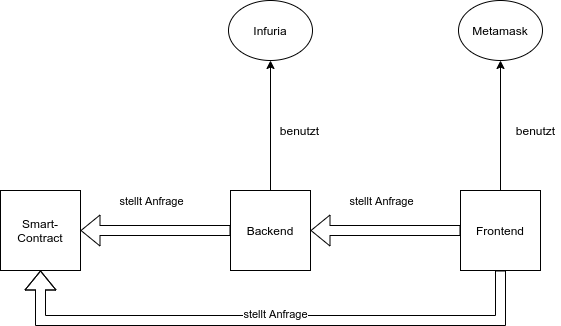
\includegraphics[width=\textwidth]{images/aufbau_PoC.png}
	\caption{Aufbau der Webanwendung}
	\label{6braun:fig:aufbau_poc}
\end{figure}\\
Die Anwendung besteht aus einem Front- und Backend, sowie einem Smart-Contract auf dem Ropsten-Testnetz, welches zum Testen von Smart-Contracts unter Ethereum dient. Sowohl Front-, als auch Backend können nicht direkt mit der Blockchain kommunizieren, sondern tun dies über sogenannte \emph{Provider}. In den folgenden Unterkapiteln sollen die einzelnen Komponenten näher erläutert werden.
\subsection{Frontend}
Das Frontend bildet den Teil der Anwendung, welcher im Browser von Nutzern läuft. Es kümmert sich um die Visualisierung und Interaktionen mit den Nutzern der Seite.
Für das Frontend wird \emph{Angular}, welches von Google in Stand gehalten wird, als Frontend genutzt. Über einen einzigen Befehl \emph{ng new} auf der Kommandozeile lässt sich eine lauffähige Webanwendung generieren, die anschließend nach belieben überarbeitet werden kann. Außerdem wird statt Javascript die Programmiersprache \emph{Typescript} genutzt, welche den Vorteil der Typsicherheit, wie sie beispielsweise aus Java bekannt ist, mitbringt. Ein letzter Vorteil unter vielen ist die Nutzung der Bibliothek \emph{RXJS}, welche eine Alternative zu bekannten Technologien wie Ajax zur Behandlung von asynchronen Funktionen bietet.
Zur Kommunikation mit der Blockchain wird die Bibliothek \emph{Ethers.js} genutzt. Sie erlaubt es Entwicklern, Anfragen an eine Blockchain-Node zu schicken, von der Transaktionen anschließend signiert und gesendet werden. Das Frontend lässt sich grob in die folgenden drei Elemente unterteilen:
\begin{itemize}
	\item Die Hauptkomponente, bestehend aus HTML-, CSS- und Typescriptdatei
	\item Der ApiService, welcher sich um die Kommunikation mit dem Backend kümmert
	\item Der BlockchainService, welcher sich um die Kommunikation mit dem Smart-Contract kümmert
\end{itemize}
Die Hauptkomponente existiert bereits nach der initialen Generierung und dient als Gerüst für die Anwendung. In Angular können Komponenten nach dem Bausteinprinzip beliebig angeordnet werden, sodass jede Komponente für einen anderen Teil der Anwendung zuständig sein kann. Auch eine hierarchische Anordnung ist möglich, sodass eine Komponente wieder andere enthält. Sogenannte \emph{Services} können durch Deklaration im Konstruktor von Komponenten genutzt werden, dies nennt man \emph{Injecting}. Services sind keine eigenständigen Komponenten, sondern stellen lediglich Funktionalitäten bereit, wie z.B. die Kommunikation mit dem Backend. Einige wichtige Funktionen der Datei \emph{app.component.ts} sollen im Folgenden erläutert werden.
\subsubsection{Konstruktor und Laden von Bildern}
\begin{lstlisting}
public constructor(private sanitizer: DomSanitizer,
private api: ApiService,
private http: HttpClient,
private formBuilder: FormBuilder,
public blockService: BlockchainService) {
	this.getImageFromApi();
	this.getImageFromApi();
}

public getImageFromApi(): void {
	this.api.getImage().subscribe((baseImage: any) => {
		const blob = new Blob([baseImage]);
		const unsafeImg = URL.createObjectURL(blob);
		
		this.upperRight === undefined ?
		this.upperRight = this.sanitizer.bypassSecurityTrustUrl(unsafeImg) :
		this.upperLeft = this.sanitizer.bypassSecurityTrustUrl(unsafeImg);
	});
}
\end{lstlisting}
Durch die Deklarationen von Klassen als Parameter des Konstruktors injiziert man diese, sodass Objekte der Klassen im Rumpf und allen anderen Methoden verwendet werden können [siehe Zeile 1-5]. So wird in der Methode \emph{getImageFromApi()} die am Objekt der Klasse ApiService die Methode \emph{getImage()} aufgerufen, die ein \emph{Observable} zurückgibt. Observables kann man sich als Objekte von asynchronen Funktionen vorstellen, über die man mithilfe der Methode \emph{subscribe()} festlegen kann, wie vorgegangen werden soll, sobald die asynchrone Funktion abgeschlossen ist [11]. Anschließend wird das rohe Bild aus der Antwort verarbeitet [12-13] und über einen ternären Operator wird entschieden, an welcher Stelle das geladene Bild eingefügt werden soll [15-17].
\subsubsection{Anpassen des Guthabens}
\begin{lstlisting}
	public augmentAds(): void {
		const id = parseInt(this.idForFunds, 10);
		const funds = parseInt(this.fundsToAdd, 10);
		
		const payment = ethers.utils.parseEther(this.fundsToAdd);
		const overrides = {
			value: payment
		};
		this.blockService.augmentAds(id, funds, overrides).then(res => {
			console.log('Funds Added!');
		});
	}
\end{lstlisting}
Die Methode \emph{augmentAds()} ist dafür da, das bestehende Guthaben für eine Anzeige zu erhöhen. 
Dafür geben Nutzer über Inputfelder auf der Seite die Id ihrer Anzeige und die Menge von Guthaben an, die sie aufstocken möchten. 
In Angular können Inputfelder direkt mit öffentlichen Variablen der Komponente verknüpft werden, sodass \emph{idForFunds} und \emph{fundsToAdd} direkt abgerufen werden können [Siehe 2-3]. Die Variable \emph{payment}, welche das Guthaben umgewandelt in Ether repräsentiert, wird initialisiert und als Wert des Felds \emph{value} in der Variable \emph{overrides} verwendet [5-8]. \emph{augmendAds()} der Klasse BlockchainService ruft die gleichnamige Methode des Smart-Contracts auf, die jedoch mit nur zwei Parametern deklariert ist. Mithilfe eines Dritten, wird in diesem Fall das Feld value des Payloads der eigentlichen Transaktion überschrieben, sodass eine Zahlung in Ether, die dem gewünschten Guthaben entspricht, entsteht [9-11]. 
\subsubsection{Ausschnitt : Hochladen eines Bildes}
\begin{lstlisting}
	// Ausschnitt aus der Methode 'onFormSubmit()'
	
	const formData = new FormData();
	formData.append('uploadedImage', 
					this.fileUploadForm.get('uploadedImage').value);
	formData.append('etherSend', 
					this.fileUploadForm.get('etherSend').value);
	
	this.blockService.sendMoney(this.fileUploadForm
	.get('etherSend').value).then((res) => {
		this.http.post<any>('http://localhost:3000/upload', formData)
		.subscribe(response => {
			console.log(response);
			// An dieser Stelle kann die Response verarbeitet werden;
		}, error => {
			console.log(error);
		});
	});
}
\end{lstlisting}
Alternativ zum direkten Verknüpfen mit einer Variable können Inputfelder Teil einer \emph{FormGroup} sein. Diese bieten Funktionalitäten, welche für Formulare nützlich sind. 
So können beispielsweise Validatoren für Felder, die bestimmte Voraussetzungen erfüllen müssen, gesetzt werden.
Über die Methode \emph{get().value} wird das Inputfeld \emph{etherSend} ausgelesen und als Parameter für die Methode \emph{sendMoney} des Services verwendet [Siehe 9-10]. Diese überschreibt genau wie augmentAds() den Payload Transaktion. Nach dem Senden wird ein Formular, bestehend aus Anzeige und Wert der Transaktion [3-7], an das Backend gesendet, in dem der Payload verarbeitet wird. Sobald eine Antwort aus dem Backend kommt, kann diese verarbeitet werden, indem man beispielsweise die Id der hochgeladenen Anzeige darstellt oder eine Fehlermeldung bei Misslingen anzeigt [11-18].
\subsection{Backend}
Das Backend ist für das Verwalten der Anzeigen zuständig und reagiert auf Anfragen aus dem Frontend. Geschrieben ist es in Javascript, wodurch der Vorteil entsteht, dass hier ebenfalls Ethers.js für die Kommunikation mit der Blockchain genutzt werden kann. Allein Javascript ist jedoch für ein Backend nicht ausreichend, denn die Programmiersprache wurde zur Ausführung im Browser entwickelt. \emph{Node.js} löst dieses Problem, indem es eine Laufzeitumgebung zur Ausführung von Javascript bereitstellt, durch die Dateien auf einer Konsole und somit einem Server ausgeführt werden können. Zusätzlich dazu wird das Framework \emph{Express.js} verwendet, um ein lauffähiges Backend, welches auf Anfragen des Frontends reagieren kann, bereitstellen zu können.
Für die Kommunikation mit dem Frontend stellt es diesem zwei Schnittstellen zur Verfügung: 
\begin{itemize}
	\item Eine Schnittstelle zum Hochladen von Anzeigen
	\item Eine Schnittstelle für das Laden von Anzeigen
\end{itemize}

\subsubsection{Hochladen einer Anzeige}
\subsubsection{Schalten einer Anzeige}

\subsection{Smart Contract}
\subsection{Provider und Deployment}
\subsubsection{Provider}
\subsubsection{Ganache}
\section{Beantwortung der Forschungsfrage}
\section{Blockchain 3.0 - Bestehende Probleme und potenzielle Lösungen}